\section{Verwendete Technologien}
\setauthor{Philipp Füreder}

\subsection*{ASP.NET Core}

Unsere Webanwendung wurde unter Verwendung der ASP.NET Core-Plattform entwickelt. 
ASP.NET Core ist ein vielseitiges, plattformübergreifendes und leistungsfähiges 
Open-Source-Framework, das zur Entwicklung moderner, internetfähigen Anwendungen geeignet ist. 
Die Ausführung findet in der .NET Core-Laufzeitumgebung statt.
ASP.NET Core bietet außerdem eine moderne und flexible Umgebung für die Entwicklung von Webanwendungen, 
die sowohl plattformübergreifend als auch hochgradig skalierbar sind. \cite{asp_dotnetcore}

Mit ASP.NET Core kann man:

\begin{itemize}

\item Webanwendungen und Webdienste, Internet-der-Dinge (IoT)-Anwendungen und 
mobile Backends entwickeln.
\item Auf verschiedene Betriebssysteme wie Windows, macOS und Linux arbeiten.
\item Anwendungen sowohl in der Cloud als auch auf lokalen Systemen bereitstellen.
\end{itemize}

Dieses Framework eröffnet somit eine breite Palette an Möglichkeiten für Entwickler, 
um moderne Anwendungen zu erstellen, die sich nahtlos mit dem Internet verbinden und 
sowohl in Cloud- als auch lokalen Umgebungen effizient betrieben werden können. \cite{asp_dotnetcore}
\newpage

\subsection*{Git}

Unsere Versionskontrolle haben wir mit Git gemacht. Git ist ein Versionskontrollsystem 
mit verteiltem Ansatz, das entworfen wurde, um sowohl kleine als auch äußerst 
umfangreiche Projekte auf schnelle und effiziente Weise zu verwalten.
Die Erlernbarkeit von Git gestaltet sich einfach, und seine geringe Systembelastung 
geht einher mit herausragender Performance. Es setzt sich von anderen Versionskontrollsystemen 
wie Subversion, CVS, Perforce und ClearCase ab, indem es Funktionen wie kosteneffiziente 
lokale „Branches“, bequeme Staging-Bereiche und vielfältige Arbeitsabläufe bietet.
Git erlaubt und begünstigt die Erstellung von mehreren unabhängigen lokalen Verzweigungen. 
Die Prozesse des Erstellens, Zusammenführens und Entfernens dieser Entwicklungsstränge 
nehmen lediglich Sekunden in Anspruch. \cite{git_introduction} \\

Git ist kostenfrei und Open-Source. Es wurde dazu entwickelt, Projekte aller 
Größenordnungen, schnell und effizient zu verwalten. 
Es zeichnet sich als Open-Source aus, da es die Anpassungsfähigkeit bietet, den Quellcode 
nach den individuellen Bedürfnissen der Nutzer/innen anzupassen. 
Mit seiner Open-Source-Natur ermöglicht Git mehreren Personen gleichzeitig an einem 
Projekt zu arbeiten und ermöglicht eine äußerst einfache und effiziente Zusammenarbeit. 
Aus diesem Grund wird Git als das herausragende Versionskontrollsystem betrachtet, 
das in der heutigen Zeit zur Verfügung steht. \cite{git_features}
\newpage

\subsection*{Docker}

Docker ist eine Plattform, welche Anwendungen gemeinsam mit ihren spezifischen Abhängigkeiten 
in Form von Containern bündelt. Dieser Ansatz gewährleistet, dass die Anwendung in 
jeder beliebigen Entwicklungsumgebung reibungslos funktioniert.
Jede einzelne Anwendung läuft in separaten Containern und verfügt über 
ihre eigenen Satz an Abhängigkeiten und Bibliotheken. Dies gewährleistet, dass jede 
Applikation in völliger Unabhängigkeit von anderen Anwendungen agiert und die Sicherheit gibt, 
dass sie Anwendungen erstellen können, welche sich nicht gegenseitig beeinträchtigen.
Wir haben in unserer Anwendung unser Frontend, Backend und die Datenbank über Docker laufen lassen.
Das heißt wir haben 3 Docker-Container benutzt. \\
 
Unter einem Container versteht man eine standardisierte Softwareeinheit, die sowohl den 
Programmcode als auch sämtliche damit verbundenen Abhängigkeiten zusammenfasst. 
Hierdurch wird sichergestellt, dass die Anwendung zuverlässig in unterschiedlichen 
Computerumgebungen ausgeführt werden kann. Ein Docker-Container-Image verkörpert eine 
autonome und ausführbare Softwareeinheit, welche sämtliche Komponenten für die Ausführung 
einer Applikation in sich trägt: den Code selbst, die Laufzeitumgebung, Systemwerkzeuge, 
Systembibliotheken und Konfigurationseinstellungen. \\

Container-Images verwandeln sich zur Laufzeit in eigenständige Container. 
Im Fall von Docker geschieht dies durch das Ausführen der Images auf der Docker Engine. 
Containerisierte Software steht sowohl für Linux- als auch für Windows-basierte Anwendungen 
zur Verfügung und gewährleistet eine gleichbleibende Ausführung, unabhängig von der genutzten 
Infrastruktur. Container schaffen eine Isolierung der Software von ihrer Umgebung und 
gewährleisten somit, dass die Anwendung konsistent arbeitet, selbst bei Unterschieden 
zwischen Entwicklungs- und Staging-Umgebungen.
\newpage
\subsection*{PostgreSQL}

Als Datenbanksystem haben wir uns für PostgreSQL entschieden, da wir bereits in anderen 
Projekten mit diesem gearbeitet haben. PostgreSQL ist Open-Source und verwendet die SQL-Sprache. 
Außerdem ist PostgreSQL auf allen gängigen Betriebssystemen kompatibel.
PostgreSQL läuft bei uns über Docker, somit haben wir nichts Zusätzliches dafür installieren müssen.
PostgreSQL ist sehr anpassbar, man kann beispielsweise eigene Datentypen 
definieren und individuelle Funktionen gestalten.\\

Datentypen in PostgreSQL:
\begin{itemize}
    \item Zahlen und Zeichen: Integer, Numeric, String, Boolean
    \item Strukturierte: Date/Time, Array, Range/Multirange
    \item Geometrisch: Point, Line, Circle, Polygon
    \item Anpassbare: Composite, Custom Types
\end{itemize}

Integrität der Daten:
\begin{itemize}
    \item UNIQUE, NOT NULL
    \item Primary Keys
    \item Foreign Keys
    \item Exclusion Constraints
    \item Explicit Locks, Advisory Locks
\end{itemize}


\newpage
\subsection*{BenchmarkDotNet (0.13.2)}

BenchmarkDotNet unterstützt Anwender/innen dabei, die Performance ihrer Methoden in 
Benchmark-Tests zu überprüfen. Ebenso ermöglicht es den Austausch von reproduzierbaren 
Messexperimenten. Diese Transformation gestaltet sich genauso unkompliziert wie die 
Erstellung von Unit-Tests. BenchmarkDotNet hilft dabei, übliche Fehler im Benchmarking-Prozess 
zu vermeiden und Nutzer zu informieren, sobald Unstimmigkeiten im Benchmark-Design oder den 
erfassten Messdaten auftreten. Die präsentierten Resultate erscheinen in einer 
nutzerfreundlichen Tabelle, die sämtliche relevanten Aspekte des Experiments herausstellt.\\
Anbei ein Beispiel von einem unserer BenchmarkDotNet-Tests:\\

\begin{lstlisting} [language={[Sharp]C},caption=BenchmarkDotNet,label=lst:impl:foo]
namespace C_SharpExample
{
    [MarkdownExporter,
        HtmlExporter,
        SimpleJob(RunStrategy.ColdStart, launchCount: 1, warmupCount: 5, targetCount: 5, id: "FastAndDirtyJob")]
    public class C_SharpTesting
    {
        [Benchmark]
        public void TestC_Sharp_Simple() => ReturnNumber();

        [Benchmark]
        public void TestC_Sharp_Sum() => MySum();

        #region C_SharpFunctions
        public static async void ReturnNumber()
        {
            var state = await CSharpScript.RunAsync("return 42;");
            Console.WriteLine(state.ReturnValue);
        }
        public static async void MySum()
        {
            var state = await CSharpScript.RunAsync("return 3 + 3;");
            Console.WriteLine(state.ReturnValue);
        }
        #endregion
    }
}
\end{lstlisting}

\newpage
\subsection*{Bogus}

Bogus haben wir in unserem Projekt für die Generierung von Fake Daten benutzt. 
Wir haben damit Schüler- und Lehrernamen erstellen lassen die wir in unserer Anwendung als 
Testdaten benutzt haben. Bogus funktioniert ausschließlich für 
.NET-Sprachen wie C\#, F\# oder VB.NET. \\

Es ist ganz unkompliziert zu verwenden. Wir haben in unserer Arbeit nur Namen generieren lassen, 
jedoch könnte man zu jedem Namen noch eine ganze Menge hinzufügen wie zum Beispiel 
Telefonnummern, E-Mail-Adressen, Wohnadressen oder auch die Herkunft.\\

Folgendes Codebeispiel zeigt die Generierung unserer Fake Daten für eine Schulklasse:\\

\begin{lstlisting} [language={[Sharp]C},caption=Bogus,label=lst:impl:foo]
            List<Student> firstStudents = new List<Student>();
                      
            #region Create Fake Students for each Schoolclass
            for (int i = 0; i < 10; i++)
            {
                var studentFaker = new Faker<Student>()
                    .RuleFor(x => x.Name, x => x.Person.FullName)
                    .Generate();
                firstStudents.Add(studentFaker);
            }
\end{lstlisting}

In der RuleFor() Methode kann man genau die Sachen angeben die man benötigt. 
In unserem Fall haben wir nur Vornamen und Nachnamen benötigt.


\newpage
\section{Aufbau}
\setauthor{Robert Freiseisen}

Um einen Überblick über die Beispielanwendung zu erhalten folgt nun ein Komponentendiagramm:

\begin{figure}[H]
    \centering
    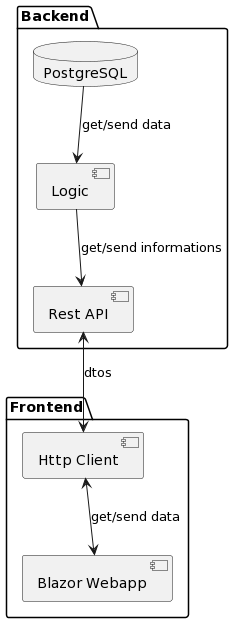
\includegraphics[scale=0.5]{pics/KomponentenDiagramm.png}
    \caption{Komponenten -- UML Diagramm}
    \label{fig:impl:KomponentenDiagramm}
\end{figure}

\newpage
Damit der Aufbau der .NET-Solution noch klarer wird ist nun die YAML-Datei dargestellt:

\lstinputlisting[style=yaml]{input-files/docker-compose.yml}

\newpage

Die verwendeten Entitäten und ihre Relationen im Backend sind in der folgenden Abbildung dargestellt.

\begin{figure}[H]
    \centering
    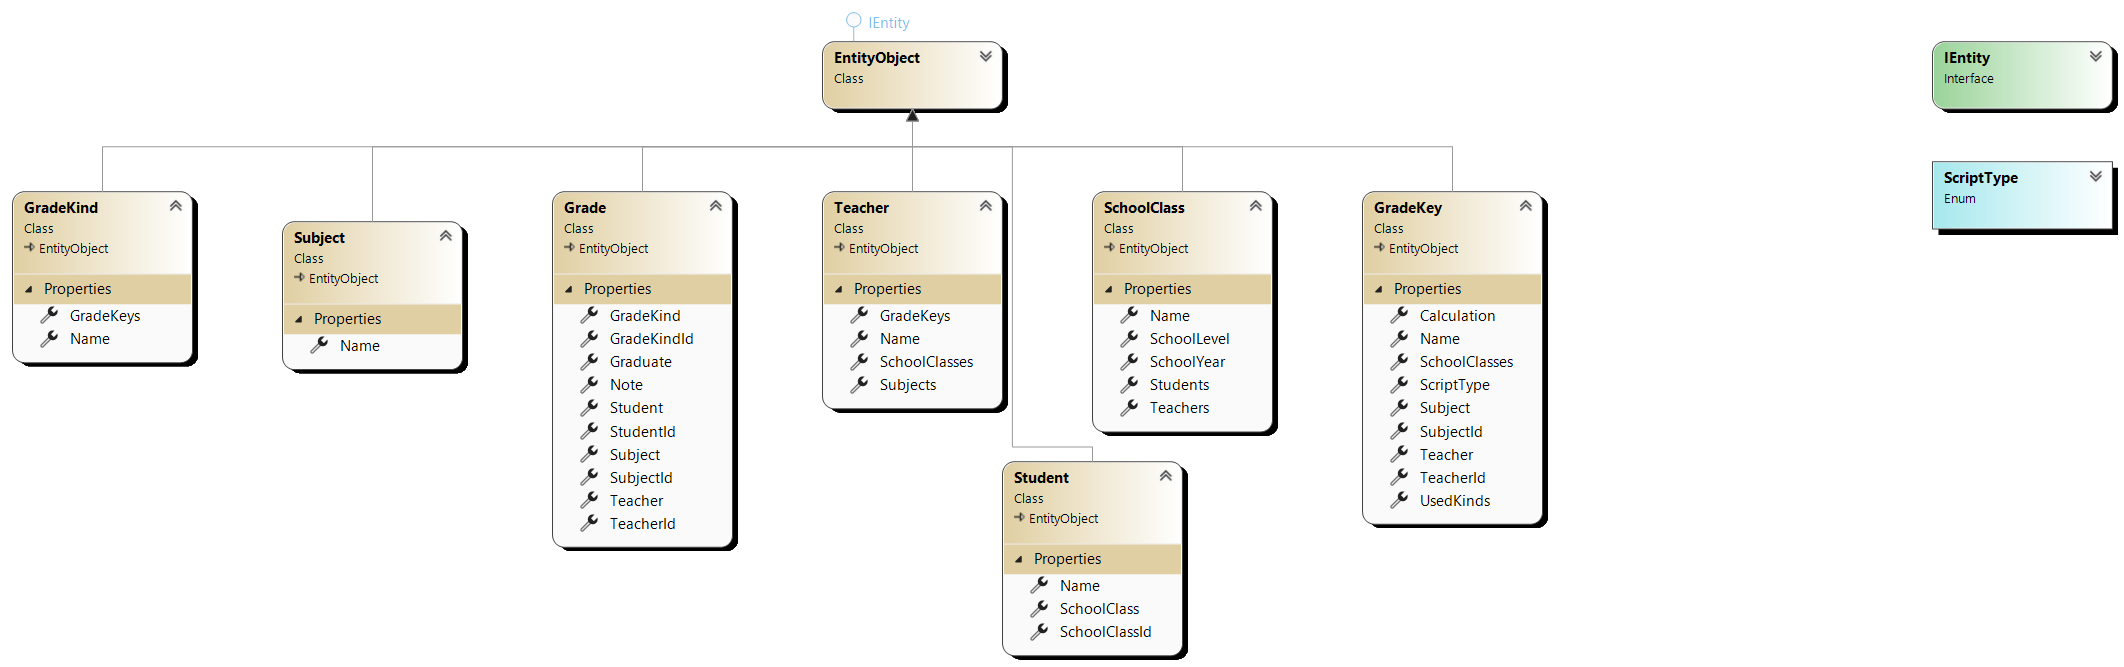
\includegraphics[scale=0.5]{pics/EntitiesClassDiagram.png}
    \caption{Entitäten -- UML Diagramm}
    \label{fig:impl:Entities}
\end{figure}

\newpage
Es gibt viele Möglichkeiten Skripte in eine Anwendung zu importieren.
Eine Möglichkeit ist die Skripte als Datei zu importieren.
Anstatt alle benötigten Daten direkt in den Code einzubetten oder sie manuell über die Befehlszeile einzugeben, 
können Entwickler eine oder mehrere Dateien als Input verwenden, die das Skript dann liest und verarbeitet.

\begin{figure}[H]
    \centering
    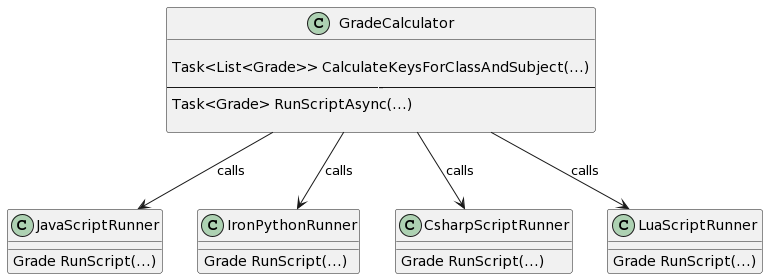
\includegraphics[scale=0.5]{pics/LogicClassDiagram.png}
    \caption{Logic Overview}
    \label{fig:impl:Logic}
\end{figure}


\newpage
Im folgenden Abschnitt  werden einige Code-Ausschnitte betrachtet, die zeigen, wie man solche Datei-Übergaben in den untersuchten Scriptsprachen realisieren kann. 

\begin{lstlisting}[language={[Sharp]C},caption=Code for Javascript,label=lst:impl:js]
    public class JavascriptRunner
    {
        public Grade RunScript(GradeKey key, List<Grade> grades)
        {
            var engine = new JintJsEngine();
            Grade result = new Grade();
            List<string>? logs = new List<string>();

            try
            {
                // Definiere eine Variable im JavaScript-Code, um die console.log-Ausgaben zu speichern
                engine.Execute("var consoleOutput = [];");

                // Definiere die console.log-Funktion im JavaScript-Code
                engine.Execute(@"
                                var console = {
                                    log: function() {
                                        consoleOutput.push(Array.from(arguments).join(' '));
                                    }
                                };
                            ");


                var gradeKindsList = JsonConvert.SerializeObject(key.UsedKinds);
                var gradesList = JsonConvert.SerializeObject(grades);

                engine.SetVariableValue("gradeKindsList", gradeKindsList);
                engine.SetVariableValue("gradesList", gradesList);

                if (key.Calculation != null)
                {
                    engine.Execute(key.Calculation);
                }

                //Die Ausgabe der console.log-Anweisungen als JSON-String
                string jsonOutput = engine.Evaluate<string>("JSON.stringify(consoleOutput)");

                // Konvertiere den JSON-String in eine Liste von strings
                if (jsonOutput != null)
                {
                    logs = JsonConvert.DeserializeObject<List<string>>(jsonOutput);

                    if (logs != null)
                    {
                        DisplayOutput(logs);   
                    }
                }

                // Get Return from Script
                var resultGrade = engine.GetVariableValue("result");

                result.Teacher = key.Teacher;
                result.Graduate = Convert.ToInt32(resultGrade);
            }
            catch (Exception)
            {
                result.Teacher = null;
                result.Graduate = 0;
            }
            return result;
        }

        private static void DisplayOutput(List<string> logs)
        {
            foreach (string output in logs)
            {
                Debug.WriteLine(output);
            }
        }
    }
\end{lstlisting}


\begin{lstlisting}[language={[Sharp]C},caption=Code for NLua,label=lst:impl:nlua]
    /// <summary>
    /// Runs lua-scripts
    /// </summary>
    public class LuaScriptRunner
    {
        private readonly Lua state;

        public LuaScriptRunner()
        {
            this.state = new Lua();
        }

        public Grade RunScript(GradeKey key, List<Grade> grades)
        {
            if (key.Calculation == string.Empty || key.UsedKinds == null || grades == null)
            {
                throw new NullReferenceException("Not enough information for Calculation");
            }

            var code = key.Calculation;

            var result = new Grade();
            try
            {
                state.DoString(code);
                state.LoadCLRPackage();
                state["grades"] = grades;
                state.DoString(@"graduate = calculate()");
                result.Teacher = key.Teacher;
                var gr = state["graduate"];
                if (gr != null) 
                {
                    result.Graduate = Convert.ToInt32(gr);
                }
            }
            catch (Exception)
            {
                throw;
            }

            return result;
        }
    }
\end{lstlisting}

\newpage

\begin{lstlisting}[language={[Sharp]C},caption=Code for CsharpScripting,label=lst:impl:csc]
    public class CsScriptRunner
    {
        public static Grade RunScript(GradeKey key, List<Grade> grades)
        {
            var result = new Grade();

            // StringWriter erstellen, um die Ausgabe des Skripts zu erfassen
            StringWriter sw = new StringWriter();

            // Console.Out umleiten
            TextWriter originalOut = Console.Out;
            Console.SetOut(sw);
            try
            {                
                dynamic script = CSScript.Evaluator
                    .ReferenceAssemblyOf(typeof(GradeKey))
                    .ReferenceAssemblyOf(typeof(Grade))
                    .CompileCode(key.Calculation)
                    .CreateObject("*");
                
                var res = script.Calculate(key, grades);
                result.Teacher = key.Teacher;              
                result.Graduate = Convert.ToInt32(res);

            }
            catch (Exception)
            {
                result.Teacher = null;
                result.Graduate = 0;
            }
            finally
            {
                // Output ausgeben
                Debug.WriteLine(sw);
            }

            return result;
        }
    }
\end{lstlisting}

\newpage
\section{Unit-Tests zur Überprüfung der Notenberechnung}
\setauthor{Philipp Füreder}

Eine der zentralen Komponenten unserer Beispielanwendung war die Implementierung von 
Skripten zur Notenberechnung in .NET-Anwendungen zur Laufzeit. Um die Zuverlässigkeit und 
Genauigkeit dieser Skripte sicherzustellen, haben wir einen Satz von Unit-Tests entwickelt 
und durchgeführt. Dieser Ansatz gewährleistet nicht nur die Integrität des Codes, 
sondern bietet auch eine robuste Basis für zukünftige Erweiterungen und Anpassungen.

\subsection*{Auswahl der Testfälle}
Die Testfälle wurden so ausgewählt, um ein breites Spektrum an Szenarien abzudecken, 
die in realen Anwendungen vorkommen könnten. Dazu gehören Standardfälle, Grenzfälle und 
auch potenzielle Fehlerzustände. Das hat uns ermöglicht, die Robustheit für unsere Test-Scripts 
umfassend zu überprüfen.

\subsection*{Ergebnisse der Unit-Tests}
Alle entwickelten Skripte zur Notenberechnung haben die Tests letztenendes erfolgreich bestanden. 
Dies gab uns ein hohes Maß an Vertrauen in die Funktionsfähigkeit und Zuverlässigkeit der 
implementierten Lösungen. Darüber hinaus haben die Tests dazu beigetragen, einige nicht 
offensichtliche Fehler und Unklarheiten im ursprünglichen Design zu identifizieren, 
die wir entsprechend beheben konnten.

\newpage
\subsection*{Testbeispiel}

In folgendem Testbeispiel haben wir ein C\#-Skript getestet:

\begin{lstlisting}[language={[Sharp]C},caption=Test for CsharpScripting,label=lst:impl:csc]
[TestMethod]
    public void CsScript_T02()
    {
        List<Grade> grades = new List<Grade>
        {
            new Grade { GradeKind = gradeKinds.Single(g => g.Name =="MAK") , Graduate = 1 },
            new Grade { GradeKind = gradeKinds.Single(g => g.Name =="MAK") , Graduate = 1 },
            new Grade { GradeKind = gradeKinds.Single(g => g.Name =="MAK") , Graduate = 1 },
            new Grade { GradeKind = gradeKinds.Single(g => g.Name =="MAK") , Graduate = 2 },
            new Grade { GradeKind = gradeKinds.Single(g => g.Name =="MAK") , Graduate = 1 },
            new Grade { GradeKind = gradeKinds.Single(g => g.Name == "TEST"), Graduate = 1},
            new Grade { GradeKind = gradeKinds.Single(g => g.Name == "TEST"), Graduate = 2},
            new Grade { GradeKind = gradeKinds.Single(g => g.Name == "TEST"), Graduate = 3},
            new Grade { GradeKind = gradeKinds.Single(g => g.Name == "TEST"), Graduate = 4},
            new Grade { GradeKind = gradeKinds.Single(g => g.Name == "TEST"), Graduate = 2},
            new Grade { GradeKind = gradeKinds.Single(g => g.Name == "HOMEWORK"), Graduate = 1},
            new Grade { GradeKind = gradeKinds.Single(g => g.Name == "HOMEWORK"), Graduate = 2},
            new Grade { GradeKind = gradeKinds.Single(g => g.Name == "HOMEWORK"), Graduate = 3},
            new Grade { GradeKind = gradeKinds.Single(g => g.Name == "HOMEWORK"), Graduate = 4},
            new Grade { GradeKind = gradeKinds.Single(g => g.Name == "HOMEWORK"), Graduate = 5},

        };

        var code = File.ReadAllText("test.cs");
        var key = new GradeKey { Name = "CsScriptTest", UsedKinds = gradeKinds, Calculation = code };

        var result = CsScriptRunner.RunScript(key, grades);

        Assert.AreEqual(2, result.Graduate, "Calculation is right");
\end{lstlisting}

Dabei beinhaltet die Liste "grades" Schulnoten von drei verschiedenen Typen:
\begin{itemize}
    \item MAK (Mitarbeitskontrolle)
    \item Test
    \item Homework
\end{itemize}


\newpage
\subsection*{Test-Skript}
Dieses Test-Skript haben wir geschrieben um die Funktionalitäten und Notenberechnungen zu testen.
Einfachheitshalber wird in diesem Skript jeder Notentyp äquivalent gerechnet.

\begin{lstlisting}[language={[Sharp]C},caption=CsharpScript-Testscript,label=lst:impl:csc]
int makCounter = 0;
int testCounter = 0;
int homeworkCounter = 0;

int mak = 0;
int test = 0;
int homework = 0;

foreach (var item in Grades)
{
    if (item.GradeKind.Name == "MAK")
    {
        mak += item.Graduate;
        makCounter++;
    }
    if (item.GradeKind.Name == "TEST")
    {
        test += item.Graduate;
        testCounter++;
    }
    if (item.GradeKind.Name == "HOMEWORK")
    {
        homework += item.Graduate;
        homeworkCounter++;
    }
}

return ((mak / makCounter) + (test / testCounter) + (homework / homeworkCounter)) / 3.0;
\end{lstlisting}

Das Skript unterscheidet zwar zwischen allen Notentypen, wertet jedoch alle gleich 
und berechnet den Durchschnitt.
